\documentclass[journal=jcisd8,manuscript=article]{achemso}

\usepackage[T1]{fontenc}
\usepackage[breaklinks]{hyperref}
\usepackage{graphicx}
% \usepackage{xcite}

\graphicspath{ {./resources/} }
\usepackage{array}
\usepackage{subfig}
\captionsetup[figure]{font=normalsize,skip=0pt}
\newcolumntype{P}[1]{>{\centering\arraybackslash}p{#1}}

% \listfiles

\newcommand*\mycommand[1]{\texttt{\emph{#1}}}
\renewcommand{\thefootnote}{\fnsymbol{footnote}}

\author{Vineeth R. Chelur}
\author{U. Deva Priyakumar}
\email{deva@iiit.ac.in}
% \phone{+91 9490441430}
\affiliation[IIIT-H]
{Center for Computational Natural Sciences \& Bioinformatics \\ International Institute of Information Technology \\ Hyderabad - 500032, India}

\title[BiRDS - Binding Residue Detection from Protein Sequences using Deep ResNets]
  {BiRDS - Binding Residue Detection from Protein Sequences using Deep ResNets
  }

\abbreviations{IR,NMR,UV}
\keywords{American Chemical Society, \LaTeX}

\begin{document}

\begin{tocentry}
    \centering
    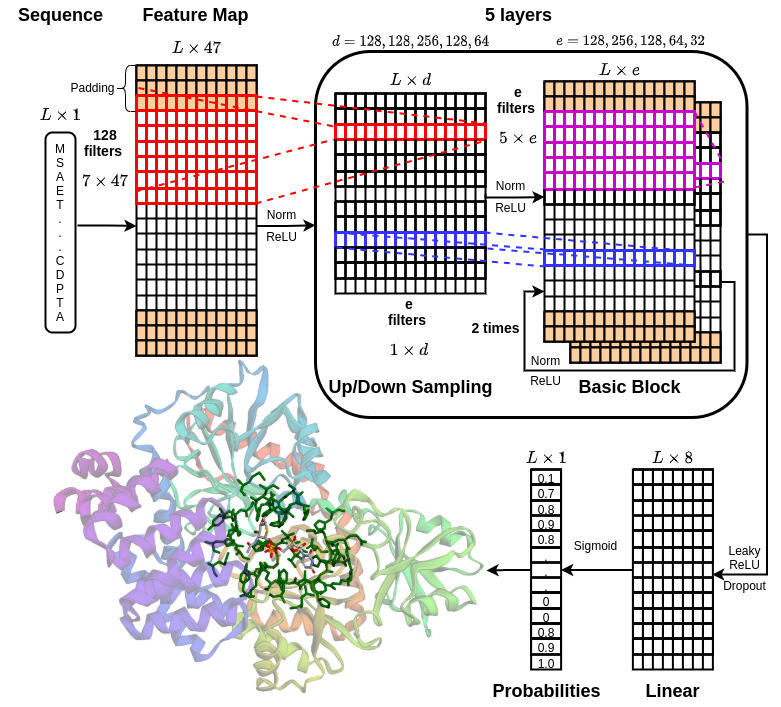
\includegraphics[width=\textwidth,height=0.15\textheight]{graphical_toc}
\end{tocentry}

\begin{abstract}
    \noindent Protein-drug interactions play important roles in many biological processes and therapeutics. Predicting the binding sites of a protein helps to discover such interactions. New drugs can be designed to optimise these interactions, improving protein function. The tertiary structure of a protein decides the binding sites available to the drug molecule, but the determination of the 3D structure is slow and expensive. Conversely, the determination of the amino acid sequence is swift and economical. Although quick and accurate prediction of the binding site using just the sequence is challenging, the application of Deep Learning, which has been hugely successful in several biochemical tasks, makes it feasible. BiRDS is a Residual Neural Network that predicts the protein's most active binding site using sequence information. SC-PDB, an annotated database of druggable binding sites, is used for training the network. Multiple Sequence Alignments of the proteins in the database are generated using DeepMSA, and features such as Position-Specific Scoring Matrix, Secondary Structure, and Relative Solvent Accessibility are extracted. During training, a weighted binary cross-entropy loss function is used to counter the substantial imbalance in the two classes of binding and non-binding residues. A novel test set SC6K is introduced to compare binding-site prediction methods. BiRDS achieves an AUROC score of 0.87, and the centre of 25\% of its predicted binding sites lie within 4{\AA} of the centre of the actual binding site.
\end{abstract}

\section{Introduction}
\quad Protein-ligand complexes are functionally important in crucial mechanisms such as DNA replication, metabolism, catalysis, defence against viruses, and signal transduction. A ligand can be any molecule that binds to the protein with high affinity where the interaction site is the active binding site of the protein. In drug design, a new drug is modelled to improve protein function after identifying a potential active binding site, thus aiding in these crucial mechanisms.

Ligand binding site prediction methods are broadly categorised into geometry-based, energy-based, template-similarity-based, traditional machine-learning-based and deep-learning-based prediction methods\cite{zhao2020exploring}. Geometry-based and energy-based methods maintain that most small ligand bindings occur in cavities on protein surfaces since large interfaces have a high affinity to small molecules. These methods locate the binding site by searching for spatial geometry or energy features by placing probes in protein structures. SITEHOUND\cite{hernandez2009sitehound} uses a carbon and phosphate probe inside a grid covering the entire protein. The grid points with higher interaction energies are clustered to determine the binding residues. A spatial geometric measurement method CURPOCKET\cite{liu2020cb} computes the curvature distribution of the protein surface and identifies clusters of concave regions. Other methods in this category include CASTp\cite{dundas2006castp}, LIGSITE\cite{hendlich1997ligsite}, VISCANA\cite{amari2006viscana}, Fpocket\cite{le2009fpocket}, and Patch-Surfer2.0\cite{zhu2015large}. While these methods are widely used, they are invalid in certain cases due to their dependence on various factors, such as the resolution of the structure determination method and the presence of both ligand groups and external molecules.

\newpage
Template-similarity-based methods consider that proteins evolved from structurally, functionally, or sequentially similar proteins, not as independent entities. S-SITE and TM-SITE\cite{yang2013protein} employ the Needleman-Wunsch algorithm to align the query protein to sequentially-similar proteins in the BioLip\cite{yang2012biolip} database, a curated database for biologically relevant ligand-protein binding interactions. The frequently-occurring binding residues in the aligned proteins form the binding residues of the query protein. Methods such as ConSurf\cite{glaser2003consurf}, FINDSITE\cite{brylinski2008threading}, 3DLigandSite\cite{wass20103dligandsite}, FunFOLD\cite{roche2011funfold}, and COFACTOR\cite{roy2012recognizing} also employ similarity searching.

3D-structure-based and template-similarity-based methods complement each other very well. Traditional machine-learning-based methods build an analytical model based on protein data to identify patterns and structural similarities. Machine learning integrates the information of both the methods and applies mathematical functions to improve prediction accuracy. P2RANK\cite{krivak2015improving}\cite{krivak2018p2rank} uses a random forest algorithm to predict ligandibility scores across the entire protein surface. Ligandibility score is the score given to a ligand for its ability to bind to specific points on the protein. The points with high scores are then clustered into a single binding pocket. SCRIBER\cite{zhang2019scriber} is a fast, sequence-based, two-layer architecture, machine learning predictor which predicts propensities of protein-binding, RNA-binding, DNA-binding, and ligand-binding residues. ConCavity\cite{capra2009predicting}, MetaPocket\cite{huang2009metapocket}, RF-Score\cite{ballester2010machine}, NsitePred\cite{chen2012prediction}, NNSCORE\cite{durrant2010nnscore}\cite{durrant2011nnscore}, LigandRFs\cite{chen2014ligandrfs}, COACH-D\cite{wu2018coach}, and Taba\cite{da2020taba} employ different machine learning models to predict the protein binding site.

Deep Learning is a subfield of machine learning based on artificial neural networks with feature learning. When a deep learning network is fed large amounts of data, it can automatically discover the representations needed for feature detection or classification. Deep learning has been hugely successful in the general areas of drug design, such as binding affinity predictions\cite{jimenez2018k,ozturk2018deepdta}, protein contact map predictions\cite{hanson2018accurate,wang2017accurate}, and protein-structure predictions\cite{senior2020improved,li2019ensembling,tiwari2020network}. Deep learning-based methods like DeepSite\cite{jimenez2017deepsite} and Kalasanty\cite{stepniewska2020improving} model binding site prediction as an image processing problem. The protein 3D structure is divided into small grids, called voxels, through a process known as voxelisation. Each voxel's specific calculated properties are used to train a deep convolutional neural network that predicts whether a voxel belongs to a binding site. DeepPocket\cite{aggarwal2021deeppocket} is a structure-based method that uses 3D Convolutional Neural Networks to generate a list of pocket probabilities. A segmentation model then elucidates shapes for the top-ranked pockets.

The tertiary structure of a protein can provide essential clues about the binding sites of a protein. Even though there have been improvements in techniques such as X-ray Crystallography, NMR Spectroscopy, and Cryo-Electron Microscopy, the determination of the three-dimensional protein structure is time-consuming and expensive. Modern DNA sequencing technologies have sped up complete DNA sequencing, and in turn, protein sequencing. The gap between the number of known protein sequences (214,406,399 UniProt sequences as of May 2021)\cite{10.1093/nar/gkaa1100} and the number of known structures (177,910 PDBs as of May 2021)\cite{berman2000protein}\cite{burley2021rcsb} is enormous. Predicting the binding site based on amino acid sequence alone is challenging. However, it helps to identify potential binding residues before the three-dimensional structure becomes available.

In this paper, a deep residual neural network (ResNet)\cite{he2016deep} is trained to predict whether an amino acid residue in the sequence belongs to the most active binding site or not. The sc-PDB database identifies this site as the binding site most suitable for docking a drug-like ligand. Features are extracted from the MSAs generated by DeepMSA\cite{zhang2020deepmsa}, whose robustness and usefulness have been studied extensively. BiRDS is trained on these features for all proteins in the training dataset. A weighted binary cross-entropy loss function is used for handling the severe class imbalance. The network outputs the final probabilities, which are converted to binary outputs. Most sequence-based prediction methods predict the binding site of a protein for specific ligands, while most popular 3D structure-based methods predict the ligandable binding sites of a protein. This paper bridges the gap between the two by providing a reliable method for predicting a protein's most active binding site from sequence information alone. SC6K, a novel test set, is used for comparing BiRDS with Kalasanty (a 3D structure-based method) and SCRIBER (a sequence-based method).

\section{Methods}
\subsection{Dataset}
\quad An annotated database of druggable binding sites from the Protein Data Bank, known as sc-PDB (v.2017)\cite{desaphy2015sc}, is used to train and validate BiRDS. The database takes samples from the Protein Data Bank\cite{berman2000protein,berman2003announcing}, creates prepared protein structures of biologically relevant protein-ligand complexes by filtering based on Uniprot annotations and prepared ligand templates. The most buried ligand, peptide or cofactor is found in the prepared structure, and the site of interaction is considered the most ligandable binding site. Thus each sample in the dataset contains the three-dimensional structure of one ligand, one protein, and one site.

The sc-PDB (v.2017) database is generally used to predict binding sites based on the available protein-ligand 3D structures. However, this paper deals with predicting the most active binding site using sequence information alone, for which the complete amino acid sequence of all the protein chains is required. The complete 3D structure is typically unavailable because some of the protein regions in the crystal under study are disordered and mobile. Hence the whole sequence cannot be extracted from the structure. Fortunately, the entire protein sequence is always available, and for this paper, it has been downloaded from the RCSB\cite{burley2021rcsb} website in FASTA file format\footnote{Some obsolete PDBs were manually tracked on RCSB, and the new PDBs that had supplanted the obsoleted PDBs were used. A list of obsoleted PDBs is provided in Supporting information}. A one-to-one mapping of the amino acids in the downloaded sequence to the amino acids in the protein's 3D structure is required to know which amino acid is a binding residue. This mapping is done by first extracting the protein sequence from the 3D structure. Next, the Needleman-Wunsch dynamic programming algorithm\cite{needleman1970general} (implemented by Zhanglab's NW-Align program\cite{NWAlign}) is utilised to align the sequence extracted from the structure file to the downloaded sequence. The protein structure file is reindexed based on this alignment to match the indices of the residues in the downloaded sequence. This reindexing allows for the labelling of binding residues in the downloaded sequence. Note that the protein sequence is the concatenation of all its chain sequences.

The training set consists of the downloaded sequence and the generated binding residue labels of every protein in the sc-PDB database, which has 17,594 PDB structures with 28,959 chain sequences, of which 9,419 are unique. For training using k-fold cross-validation, we must ensure that no two folds have proteins with sequence similarity greater than 25\% to avoid data leakage between the training and validation set during network training. Hence, the pairwise sequence similarity of the 9,419 unique chain sequences was calculated using BLASTP (part of the BLAST$^+$\cite{camacho2009blast+} package from NCBI). SiLiX\cite{miele2011ultra} package clustered these unique sequences into families with greater than 25\% sequence similarity and over 80\% overlap, leading to the creation of 2,039 clusters of chain sequences. Since BiRDS predicts the most active binding site of the complete protein, the protein sequence must also be clustered. The Union-Find algorithm\cite{kozen1992union} using a disjoint-set data structure was employed to make this clustering, where all the chains of a protein and their corresponding cluster were put in a single set, creating 1,744 sets. Protein sequences longer than 4,096 residues were removed. An equal sum K-partition algorithm put these sets into ten folds for cross-validation. One set had 2,009 proteins and was reduced to 1,642 to split the sets into ten even folds. Finally, this gave 16,450 proteins belonging to the training set, with each fold containing 1,645 proteins.

A separate test set SC6K was constructed using the PDB structures from January 2018 to February 2020. All PDBs with at least one ligand were run through pdbconv program from the IChem Toolkit\cite{da2018ichem}. The program used the exact filtering mechanism and site selection method as the sc-PDB\cite{desaphy2015sc} database. The entire test set consists of 2,274 PDB structures with 3,434 chain sequences, of which 1,889 are unique. However, there should be no data leakage between the test and training sets. Hence, the pairwise sequence similarity of the 1,889 test chain sequences with the 9,419 training chain sequences was calculated using BLASTP. Sequences with greater than 25\% similarity and over 80\% overlap were removed from the test set, giving a set of 576 chain sequences. Proteins with all their chain sequences in this set were considered for the reduced test set, leading to a final count of 530 protein sequences.

\subsubsection{MSA Generation}
\label{msa_generation}
\quad Collections of multiple homologous sequences (called Multiple Sequence Alignments or MSAs) can provide critical information for modelling the structure and function of unknown proteins. DeepMSA\cite{zhang2020deepmsa} is an open-source method for sensitive MSA construction, which has homologous sequences and alignments created from multiple sources of databases through complementary hidden Markov model algorithms. DeepMSA profiles provided statistically significant improvements in residue-level contact prediction, homologous structure identification and secondary structure prediction. These improvements were achieved without retraining the parameters and neural-network models.

The search for alignments is done in 2 stages. In stage 1, the query sequence is searched against the UniClust30\cite{mirdita2017uniclust} database using HHBlits from HH-suite\cite{remmert2012hhblits} (v2.0.16). If the number of effective sequences is $<$ 128, Stage 2 is performed where the query sequence is searched against the Uniref50\cite{suzek2015uniref} database using JackHMMER from HMMER\cite{johnson2010hidden} (v3.1b2). Full-length sequences are extracted from the JackHMMER raw hits and converted into a custom HHBlits format database. HHBlits is applied to jump-start the search from the Stage 1 sequence MSAs against this custom database.

\subsection{Features}
\quad The MSAs were generated for the unique chain sequences in the training(9,419), and test(1,889) sets using the method described in \nameref{msa_generation} and stored in PSICOV\cite{jones2012psicov} .aln format. The most commonly used features in sequence-based predictions were used. Token embeddings, Positional embeddings, and Segment embeddings were extracted from the sequence, while Position Specific Scoring Matrix, Information Content, Secondary Structure, and Solvent Accessibility were extracted from the generated, high-quality MSAs. The process for creating the feature map is shown in Figure \ref{fig:feature_map}

\begin{figure}
    \centering
    \noindent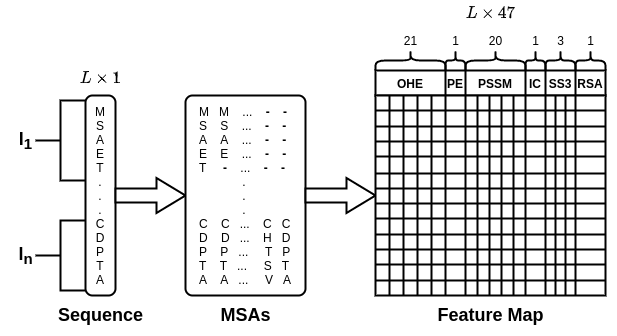
\includegraphics[width=0.8\textwidth]{feature_map}
    \caption{\centering The process used for generating the feature map of BiRDS framework. Token, positional and segment embeddings are generated using just the sequence information. The features extracted from the MSAs of the individual protein chains created using DeepMSA, are concatenated to form the protein feature map}
    \label{fig:feature_map}
\end{figure}

\subsubsection{Token Embedding, Positional Embedding and Segment Embedding}
\quad There are 21 amino acids in the protein vocabulary of BiRDS, with the 20 standard amino acids labelled in alphabetical order from 1 to 20 and X, representing all non-standard amino acids, labelled as 0. Token embeddings help the model differentiate between the different types of amino acids. It is generated by an Encoding layer that uses the vocabulary label of each amino acid in the sequence. Positional Embeddings (PE) carry information about the absolute position of the amino acids in the sequence. Using the positional encoding layer of a Transformer network\cite{vaswani2017attention}, these embeddings were unique for each position and generalised to long sequences without extra effort. A segment embedding was generated by using the chain number to which an amino acid belongs, to allow the model to differentiate between the multiple chains of a protein.

\subsubsection{Position-Specific Scoring Matrix and Information Content}
\quad Position-Specific Scoring Matrix (PSSM) is a commonly used representation of patterns in biological sequences, derived as the log-likelihood of the probability that a particular amino acid occurs at a specific position. The PSSMs were derived from MSAs using Easel\cite{potter2018hmmer} and Heinikoff position-based weights so that similar sequences collectively contributed less to PSSM probabilities than diverse sequences. The information content (IC) of a PSSM gives an idea about how different the PSSM is from a uniform distribution. IC was also derived using Easel.

\subsubsection{Secondary Structure and Solvent Accessibility}
\quad The secondary structure is defined by the pattern of hydrogen bonds formed between the amino hydrogen and carboxyl oxygen atoms in the peptide backbone. It gives an idea of the three-dimensional structure of the protein. The secondary structural elements are alpha helices, beta sheets and turns. PSIPRED (v4.0)\cite{jones1999protein} was used to predict the probability of each state of the 3-state secondary structure (SS3) for every amino acid in the sequence. The solvent-accessible surface area is the surface area of a biomolecule accessible to a solvent. SOLVPRED from MetaPSICOV 2.0\cite{jones2015metapsicov} was used to predict the every amino acid's relative solvent accessibility (RSA). RSA can be calculated as \\ ${RSA} = {ASA} / {MaxASA}$, where ASA is the solvent-accessible surface area, and MaxASA is the maximum possible solvent accessible surface area for the amino acid residue.

\subsection{Model}
\subsubsection{BiRDS Architecture}
\label{birds_architecture}
\quad A Convolutional Neural Network (CNN) is a Deep Learning algorithm that can take an image as input, assign importance (learnable weights and biases) to various aspects/objects in the image, and differentiate one from the other. When multiple CNN layers are stacked on top of each other, Deep Neural Networks (DNNs) are formed. DNNs are challenging to train because of the vanishing gradient problem where the gradients become so small that the network's weights do not change, preventing further training. With the introduction of skip connections (shortcuts to jump over some layers) in CNNs, the vanishing gradient problem is avoided. CNNs with skip connections are known as Residual Neural Networks or ResNets\cite{he2016deep}. ResNets use representation learning to extract the most important features for classification. They can also model long-range interactions and have been hugely successful in Computational Natural Sciences\cite{senior2020improved}. The architecture of the deep Residual Neural Network used here is shown in Figure \ref{fig:architecture}.

Each sample protein in the dataset consists of one or more protein sequences. Let the length of the sequences be $l_1, ..., l_n$. Features are generated for each sequence in the protein (ordered by chain ID in PDB), leading to multiple vectors of shape $[l_i, 47]$ for the $i^{th}$ sequence. These generated features are combined through simple concatenation, giving a final feature vector of shape $[L, 47]$ as input to the model, where $L = l_1 + ... + l_n$.

\begin{figure}
    \centering
    \noindent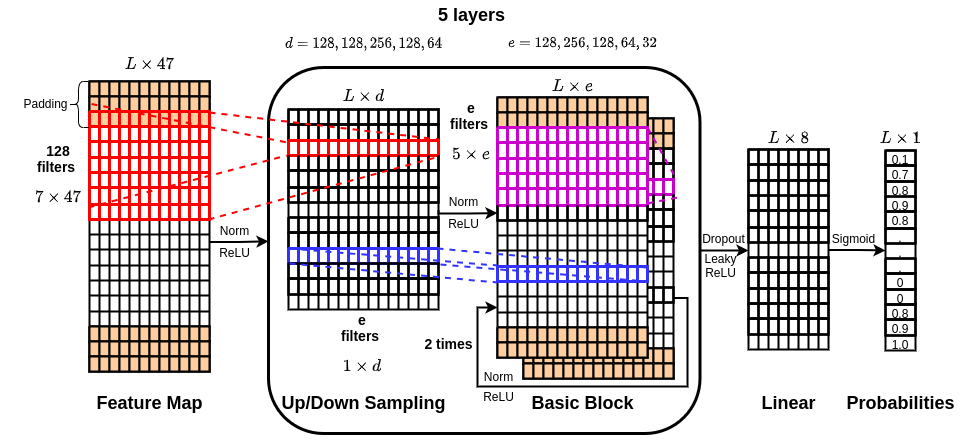
\includegraphics[scale=0.5]{architecture}
    \caption{\centering Architecture of the deep learning model, BiRDS}
    \label{fig:architecture}
\end{figure}

\newpage
The feature vector is passed through the first level, consisting of a 1D convolutional layer with 128 filters of size 7, batch normalisation layer and ReLU (Rectified Linear Unit) activation function. The input is padded with zeroes to ensure that the length of the output vector remains the same. The filters of this layer stride along the length of the protein, considering the features of the three prior amino acids, the current amino acid, and the three subsequent amino acids (totalling 7). This stride allows for the extraction of the required information of the current amino acid based on the features of nearby amino acids.

The following five levels contain an up(down)sampling layer and two basic blocks. A basic block consists of a 1D convolutional layer, a batch normalisation layer, a ReLU activation function, a second 1D convolutional layer, a second batch normalisation layer, and a final ReLU activation function. The ResNet skip connection is made after the final ReLU activation, where the initial input to the first basic block is added to the output of the final ReLU activation. Usually, the input received by the first basic block will not match its required input size. Hence, an up(down)sampling layer ensures that the input to the first block has the required shape. The output of size $L \times d$ from the first level runs through $e$ filters of size $1 \times d$ of the up(down)sampling layer to generate a vector of size $L \times e$. This vector is passed to the first basic block, which follows a similar stride policy as the first level but with a window size of 5. The process is repeated with the second basic block, and its output is sent back to the up(down)sampling layer. This process is repeated five times, with $d$ going from $128 \to 128 \to 256 \to 128 \to 64$ and $e$ going from $128 \to 256 \to 128 \to 64 \to 32$. The multiple levels capture the long-range dependencies of amino acids since the filters help propagate information of one amino acid through its neighbours.

The last two levels contain simple, linear, fully connected artificial neural networks. The penultimate level has a LeakyReLU activation function with dropout to prevent sparse gradients. A sigmoid function at the end ensures that the model outputs values between $[0, 1]$, resulting in a vector of size $L$ (length of the protein), denoting the probabilities of a residue being a part of the binding site.

\subsubsection{Loss Function}
\quad There is a substantial imbalance in the two classes of binding and non-binding residues in this classification problem, where the percentage of binding residues is only 6\%. Hence, a weighted binary cross-entropy loss function was used to train the model.
$$L(\hat{y}, y) = -(\alpha\hat{y}\log(y) + (1-\hat{y})\log(1-y))$$ \quad$\hat{y}$ is the vector of true labels, $y$ is the model output probabilities, and $\alpha$ is the weight assigned to the rare class.

$\alpha$ heavily penalises the model if it incorrectly predicts binding residues as non-binding. $\alpha$ is calculated on the fly for every batch of inputs using $\alpha = \frac{n_{nbr}}{n_{br}}$, where $n_{nbr}$ is the total number of non-binding residues in the batch and $n_{br}$ is the total number of binding residues in the batch.

\subsubsection{Implementation}
\quad The model is implemented using PyTorch Lightning\cite{falcon2019pytorch}, a wrapper on the popular open-source deep-learning library, PyTorch\cite{paszke2019pytorch}. The model is trained in batches using an Adam Optimiser with the ReduceLROnPlateau scheduler and a learning rate warm-up where the learning rate is gradually increased to the actual learning rate. The implementation can be found at \href{https://github.com/devalab/BiRDS}{https://github.com/devalab/BiRDS}.

\section{Results and Discussion}
\quad Ten models with the architecture described in \nameref{birds_architecture} were trained through ten-fold cross-validation, where one fold formed the validation set while the remaining folds formed the training set in each iteration. The validation results are provided in Table \ref{tab:results} and the sum of confusion matrices in Figure \ref{fig:valid_cm}. The Receiver Operating Characteristics (ROC) curve and the Precision-Recall (PR) curve of the models on their validation sets is provided in Figure \ref{fig:valid_roc_prc}. The description of the various metrics is provided in Supplementary Information.

\begin{table}
    \centering
    \begin{tabular}{| P{2.9cm} | P{1.75cm} | P{1.75cm} | P{1.75cm} | P{1.75cm} | P{1.75cm} | P{1.75cm} |}
        \hline
        Dataset        & MCC   & ACC   & F1    & IoU   & PPV   & TPR   \\
        \hline
        Fold 1         & 0.354 & 0.920 & 0.394 & 0.582 & 0.359 & 0.437 \\
        Fold 2         & 0.606 & 0.931 & 0.633 & 0.695 & 0.545 & 0.755 \\
        Fold 3         & 0.521 & 0.896 & 0.565 & 0.641 & 0.474 & 0.700 \\
        Fold 4         & 0.270 & 0.898 & 0.323 & 0.544 & 0.296 & 0.355 \\
        Fold 5         & 0.324 & 0.892 & 0.367 & 0.556 & 0.293 & 0.490 \\
        Fold 6         & 0.338 & 0.884 & 0.373 & 0.555 & 0.282 & 0.550 \\
        Fold 7         & 0.324 & 0.902 & 0.368 & 0.562 & 0.309 & 0.456 \\
        Fold 8         & 0.340 & 0.924 & 0.380 & 0.578 & 0.355 & 0.407 \\
        Fold 9         & 0.380 & 0.918 & 0.421 & 0.591 & 0.378 & 0.475 \\
        Fold 10        & 0.355 & 0.917 & 0.391 & 0.579 & 0.332 & 0.476 \\
        Test (Full)    & 0.568 & 0.940 & 0.589 & 0.677 & 0.502 & 0.713 \\
        Test (Reduced) & 0.440 & 0.951 & 0.464 & 0.626 & 0.497 & 0.436 \\
        \hline
    \end{tabular}
    \caption{\label{tab:results} Validation and test results}
\end{table}

\newpage
The model predictions were also mapped back to the available 3D structures of proteins for DCC calculation. DCC is the distance between the centre of the predicted binding pocket and the centre of the actual binding pocket. It is commonly used for evaluating 3D-structure based models. The success rate of DCC is defined as the fraction of predictions below a given threshold. Pockets with DCC below 4{\AA} are considered to be correctly predicted. Figure \ref{fig:valid_dcc} denotes the success rate plot of the models' predictions on their validation set for various thresholds of the DCC metric. The success rate ranges from 15\% to 75\% when the threshold is 4{\AA}. Fold 2 and Fold 3 models performed well on their validation sets since they contained only 1 to 5 protein families with similar sequence patterns. The presence of only a few families in these folds is due to the equal sum partition algorithm used to create these folds. It is a greedy algorithm that combines as many large clusters as possible, thus causing large families to appear in a single fold.

\begin{figure}%
    \centering
    \subfloat[\centering Sum of confusion matrices]{{ \noindent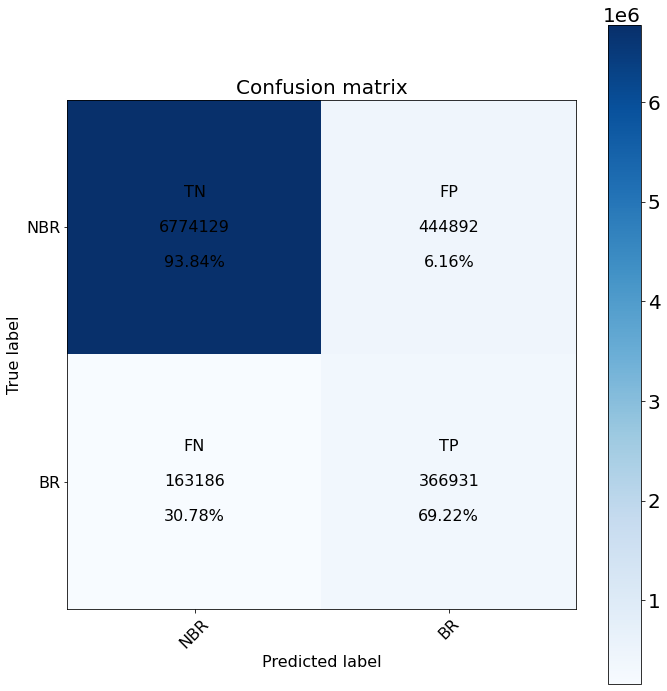
\includegraphics[width=0.45\textwidth]{valid_cm.png} \label{fig:valid_cm}}}%
    \subfloat[\centering Success rate plot for various DCC thresholds]{{ \noindent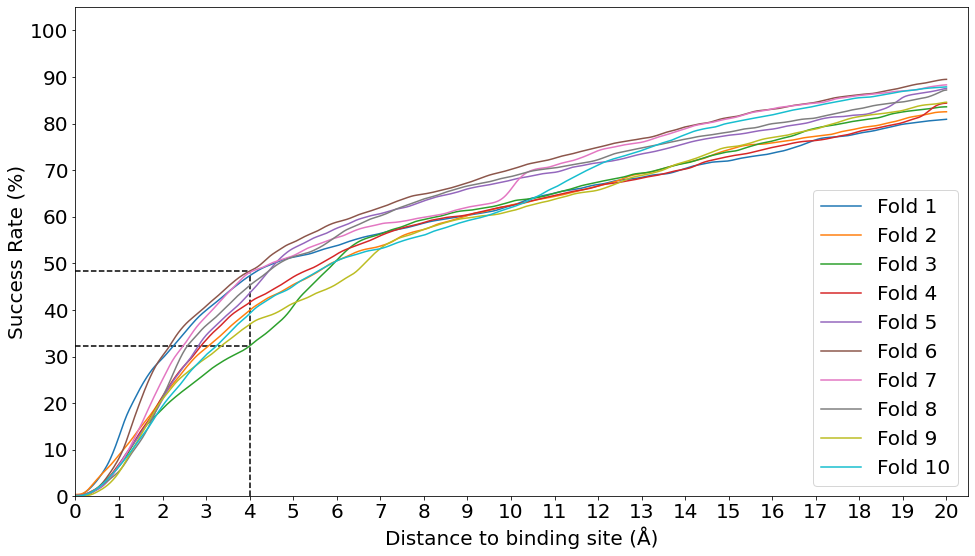
\includegraphics[width=0.55\textwidth]{valid_dcc.png} \label{fig:valid_dcc}}}%
    \vspace{1em}
    \caption{\centering Results of the ten models on their corresponding validation sets}%
    \label{fig:valid_results}%
\end{figure}

\begin{figure}%
    \centering
    \subfloat{{ \noindent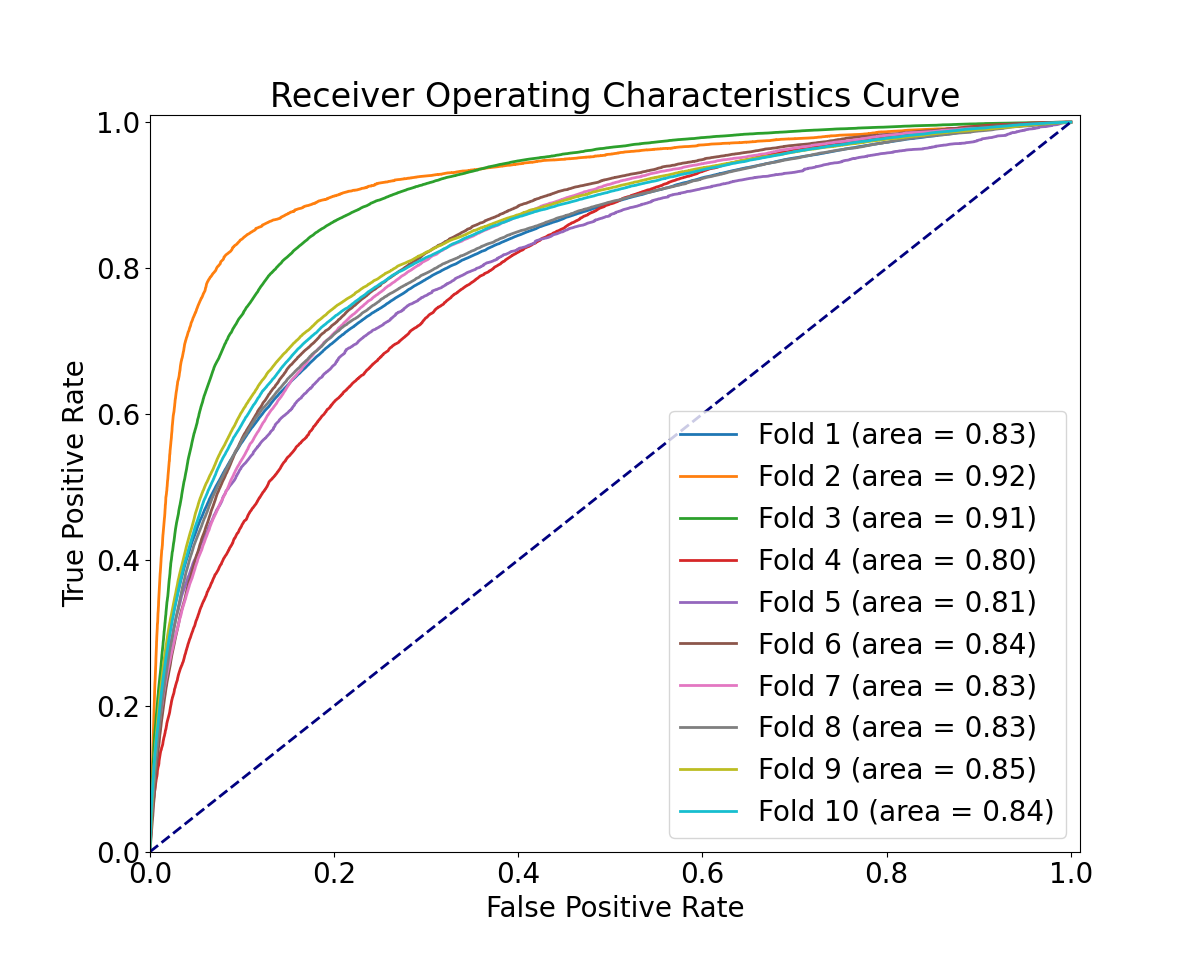
\includegraphics[width=0.52\textwidth]{valid_roc.png} \label{fig:valid_roc}}}%
    \subfloat{{ \noindent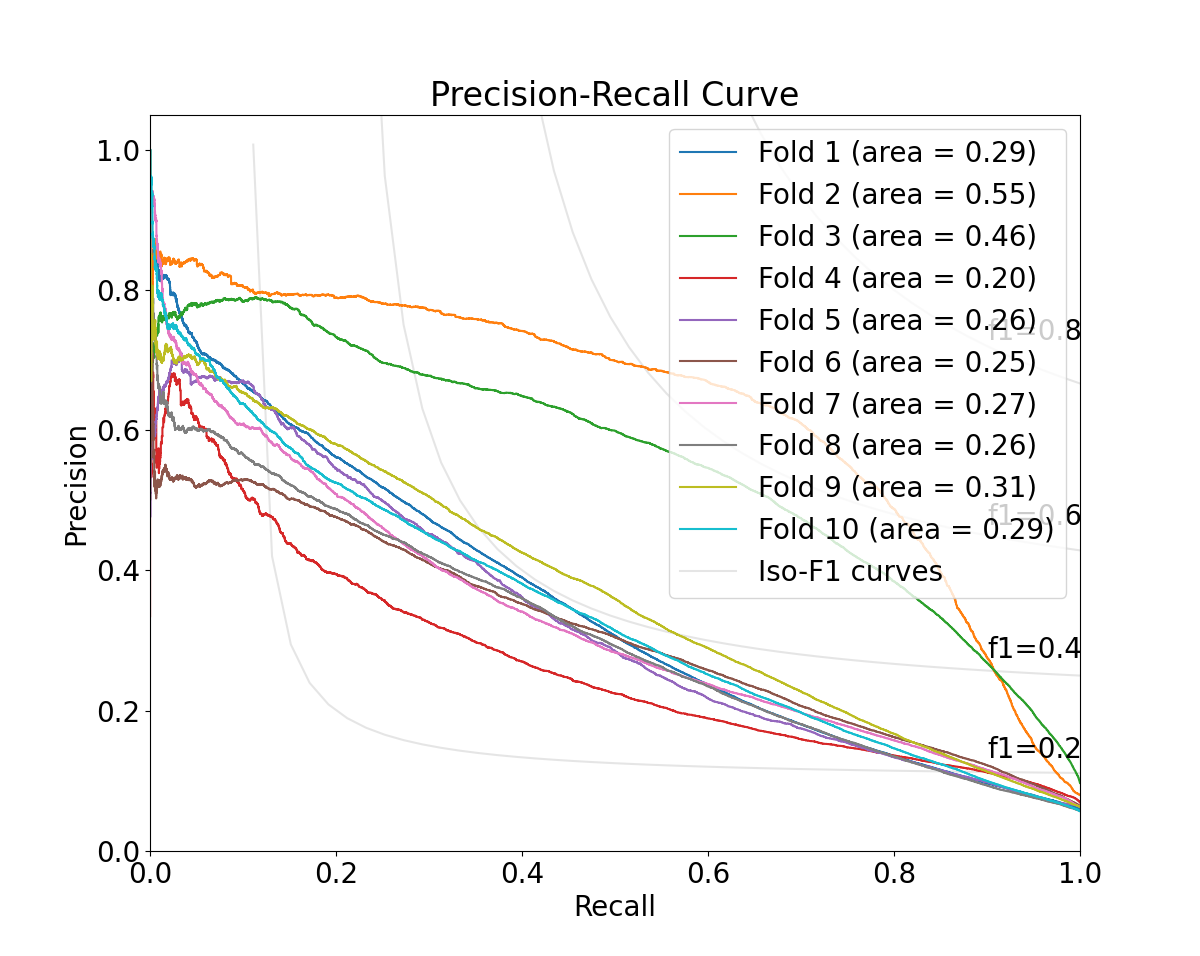
\includegraphics[width=0.52\textwidth]{valid_prc.png} \label{fig:valid_prc}}}%
    \vspace{1em}
    \caption{\centering ROC and PR curves of the ten models on their corresponding validation sets }%
    \label{fig:valid_roc_prc}%
\end{figure}

The ten trained models are run on the full and reduced test sets for testing. The models come to a consensus if five or more models predict a residue as belonging to the most active binding site of the proteins in a set. The test results, both full and reduced, are provided in Table \ref{tab:results} and the confusion matrices in Figure \ref{fig:test_cm}.

\begin{figure}%
    \centering
    \subfloat[\centering Reduced test set]{{ \label{fig:test_reduced_cm} 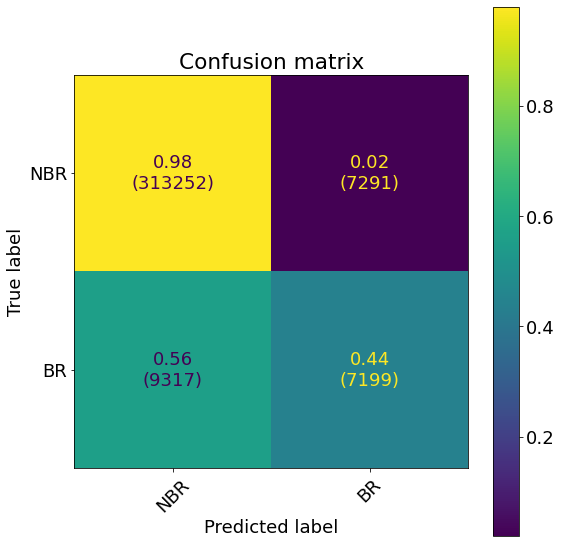
\includegraphics[width=0.45\textwidth]{test_reduced_cm.png} }}%
    \subfloat[\centering Full test set]{{ \label{fig:test_full_cm} 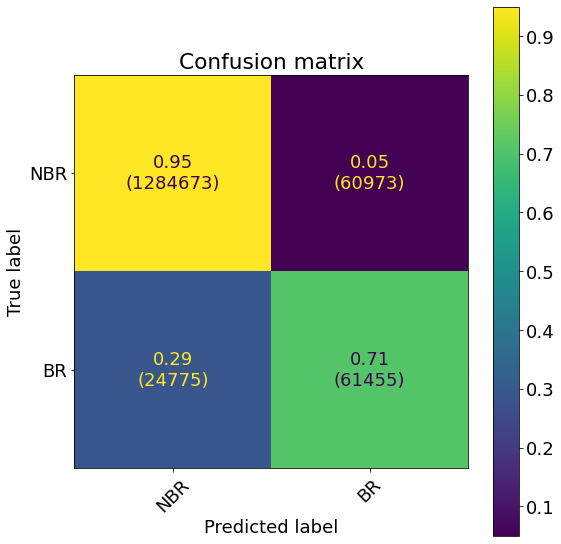
\includegraphics[width=0.45\textwidth]{test_full_cm.png} }}%
    \vspace{1em}
    \caption{\centering Confusion matrix on the test sets after consensus among models}%
    \label{fig:test_cm}%
\end{figure}

\newpage
The performance of BiRDS on the novel SC6K test set was compared against Kalasanty\cite{stepniewska2020improving} and SCRIBER\cite{zhang2019scriber}. Kalasanty is a 3D-structure-based method that uses a U-Net architecture\cite{ronneberger2015u} capable of protein binding site segmentation. The full test set was run on Kalasanty using their open-source code, and the DCC metric was calculated for the predicted pocket. The success rate plot of DCC is shown in Figure \ref{fig:test_dcc}. BiRDS performs on par with Kalasanty on the full test set, which will have a lot of sequences similar to the training data. However, the performance on the reduced test set shows Kalasanty outperforming BiRDS. Nevertheless, BiRDS still performs well on the reduced test set for a sequence-based predictor, achieving a success rate of 25\% at a 4{\AA} cutoff for DCC. In other words, for 25\% of the test data, the model has predicted the binding site such that the centre of the predicted binding site is within 4{\AA} of the centre of the most ligandable binding site. As the threshold of DCC increases, the success rate also naturally increases. It should be noted that if the model predicts the whole binding site correctly and misses out on a couple of residues or predicts more residues, the centre of the predicted binding site may shift significantly.

\begin{figure}
    \centering
    \noindent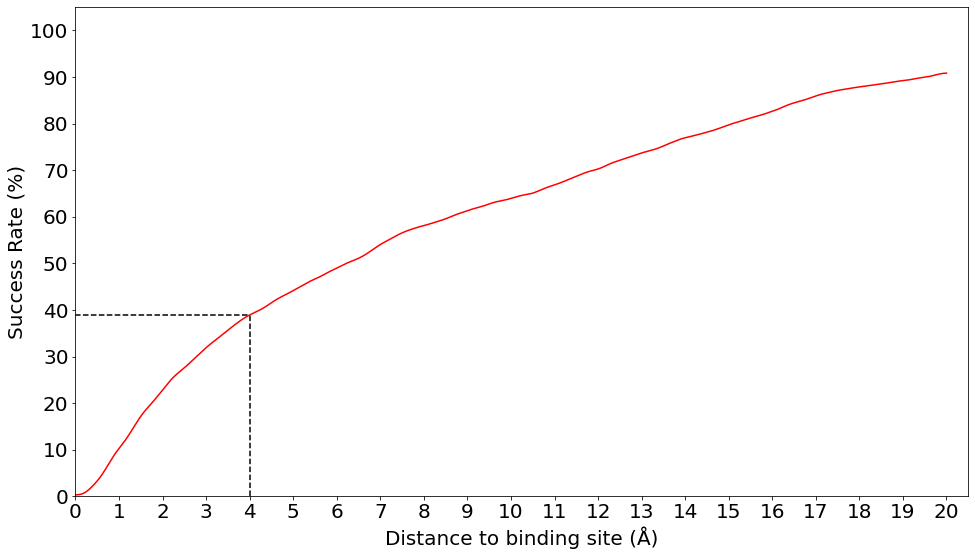
\includegraphics[width=0.6\textwidth]{test_dcc.png}
    \caption{\centering Success rate plot for various DCC thresholds on the test set after averaging the predictions of the 10 models}
    \label{fig:test_dcc}
\end{figure}

SCRIBER is a sequence-based, two-layer architecture, machine learning predictor which predicts propensities of protein-binding, RNA-binding, DNA-binding, and ligand-binding residues. The predictor was trained on individual chain sequences of a protein, based on their Uniprot IDs. For a fair comparison with BiRDS and to speed up prediction time on their webserver, the 1,889 unique chain sequences of the test set were filtered; sequences with length greater than 1,024 and sequences with sequence similarity greater than 25\% and over 80\% overlap with the SCRIBER training set and SC6K test set were removed. SCRIBER predictions of RNA-binding, DNA-binding and ligand-binding residue propensities on the final 521 sequences were averaged and considered for comparison. The Receiver Operating Characteristic (ROC) curve and the Precision-Recall (PR) curve of BiRDS on the full and reduced test set, and SCRIBER on the 521 sequences, is shown in Figure \ref{fig:test_roc_prc}.

\begin{figure}%
    \centering
    \subfloat{{ \noindent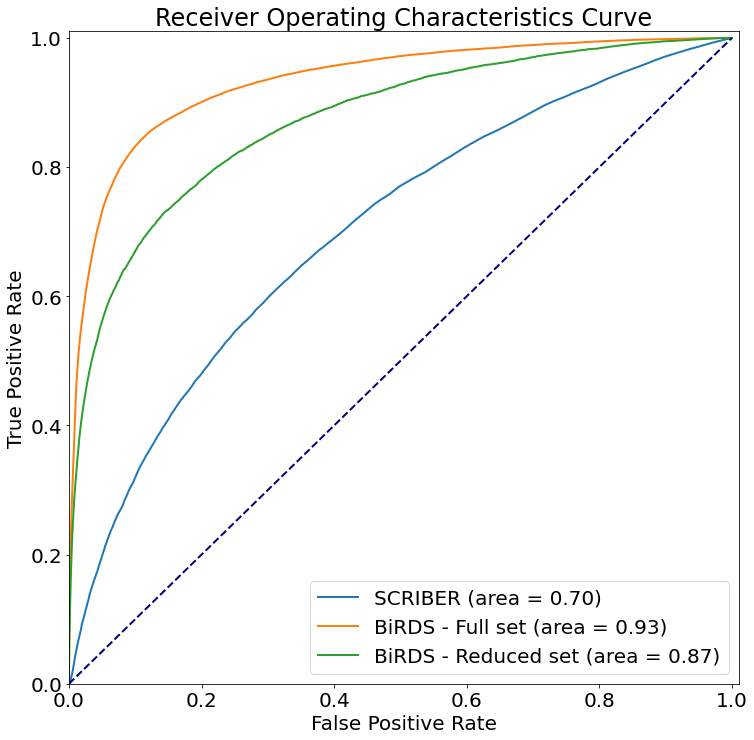
\includegraphics[width=0.5\textwidth]{test_roc.png} \label{fig:test_roc}}}%
    \subfloat{{ \noindent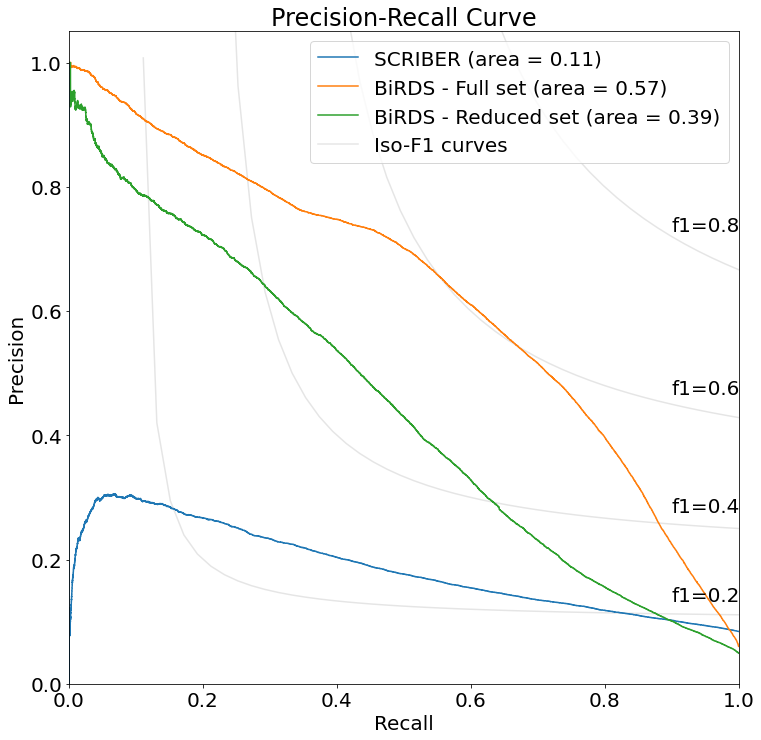
\includegraphics[width=0.5\textwidth]{test_prc.png} \label{fig:test_prc}}}%
    \vspace{1em}
    \caption{\centering ROC and PR curve of BiRDS and SCRIBER on the test sets}%
    \label{fig:test_roc_prc}%
\end{figure}

\newpage
A variety of more complex deep-learning models were trained to improve predictions. As described in the paper by \citeauthor{cui2020conan}, a Complementary Generative Adversarial Network (CGAN) was implemented to mitigate the substantial imbalance in the prediction classes. However, a simple weighted binary cross-entropy loss function worked better than a CGAN with focal loss. A Deep Bidirectional Encoder Representations from Transformers (BERT)\cite{devlin2018bert}, a state-of-the-art model for token classification problems in NLP, was also implemented. It performed on par with the current BiRDS model but led to longer training times. Several different features to improve performance were also tried. Task Assessing Protein Embeddings (TAPE)\cite{rao2019evaluating} provided trained deep learning models which produced an embedding representation of the protein sequence input. The trained TAPE transformer model was added along with BiRDS architecture, but the training could not proceed due to a large-sized feature map and insufficient GPU memory. SPOT-1D\cite{hanson2019improving} is a sequence-based predictor for predicting secondary structure, backbone angles, solvent accessibility and contact numbers by using predicted contact maps. These predictions were used as inputs to BiRDS but did not provide any improvement over the features extracted from Deep MSAs. An ablation study to identify the importance of the features currently used by BiRDS can be found in Supplementary Information.

\quad Some case studies were undertaken to show that the model's performance is good, but the metrics do not rate it well due to the limitations of the dataset. The aggregated predictions of the ten models on the test set were mapped back to the three-dimensional structure of the protein-ligand complex. 3Dmol.js\cite{rego20153dmol}, a modern, object-oriented Javascript library for visualising molecular data, was used to visualise the protein's surface, with coloured residues representing the predicted and actual binding residues. In the following examples, red indicates an incorrect prediction of a non-binding residue as binding, blue indicates a binding residue that was not predicted as binding, and green indicates a correct prediction.

\newpage
In Figure \ref{fig:6fad}, BiRDS seems to incorrectly predict all the binding residues for 6FAD\cite{tunnicliffe2019molecular}. However, it is predicting another binding site of the protein. The sc-PDB\cite{desaphy2015sc} dataset was generated through a series of filters, and the residues surrounding the most buried ligand was selected to be the most ligandable binding site. This selection, unfortunately, is a flaw of the dataset and the method used for predictions. There is no right way to cover cases like these where the model needs to be penalised less when it predicts a binding site that is not the most ligandable binding site. Hence, the evaluation metrics will generally give an abysmal score for such cases.
\begin{figure}
    \centering
    \noindent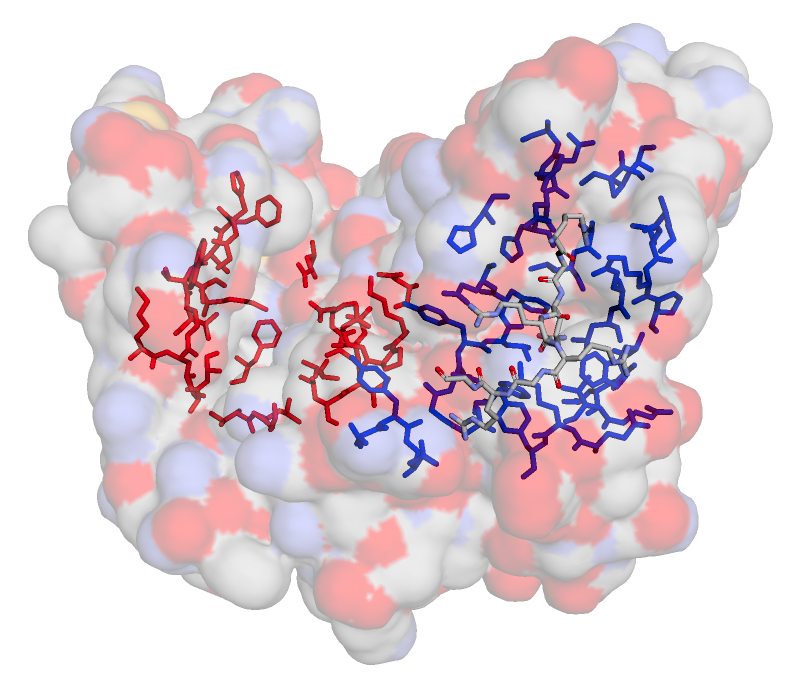
\includegraphics[width=0.6\textwidth]{6fad.png}
    \caption{\centering 6FAD - BiRDS seems to be incorrectly predicting the actual binding site (in blue), when in reality, it is predicting another binding site of the protein (in red)}
    \label{fig:6fad}
\end{figure}

Figure \ref{fig:6isp} shows 6ISP\cite{cen2019artificial}, where BiRDS predicts individual binding sites of two same sequence chains of the protein. However, the model finds it challenging to predict the binding site created due to the interaction between the two chains. This may likely be due to the way the input features are generated. A simple concatenation of the features of individual chains to generate the protein sequence features is insufficient as it does not provide any information about the interaction among the multiple chains. These interactions scarcely occur in the training set, making it hard for BiRDS to learn.
\begin{figure}
    \centering
    \noindent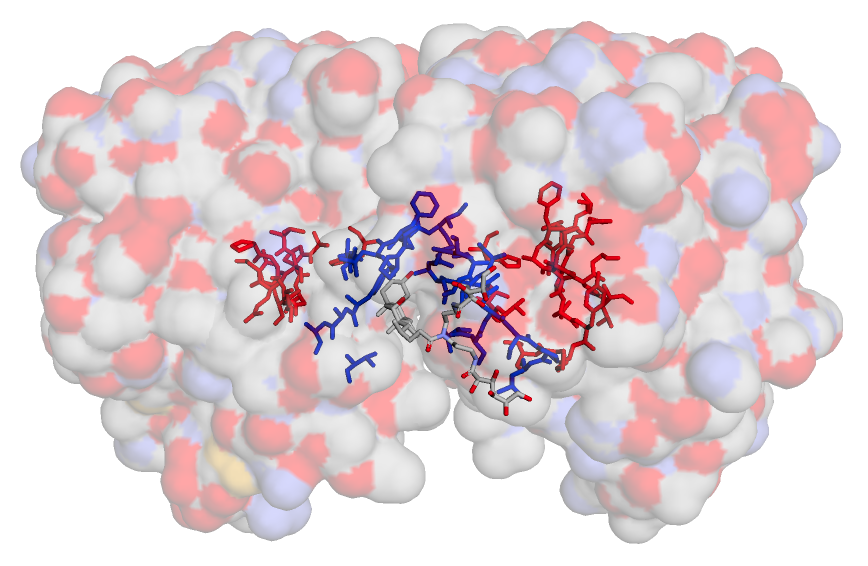
\includegraphics[width=0.6\textwidth]{6isp.png}
    \caption{\centering 6ISP - BiRDS is able to predict the binding site of individual chains (in red), but not the binding site formed due to the interaction between chains (in blue)}
    \label{fig:6isp}
\end{figure}

\begin{figure}
    \centering
    \noindent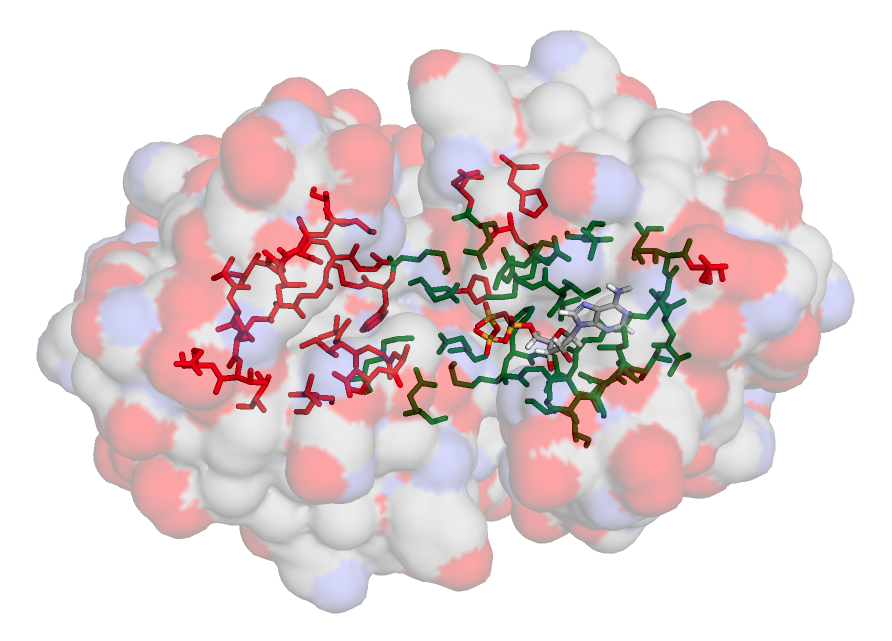
\includegraphics[width=0.6\textwidth]{6s2j.png}
    \caption{\centering 6S2J - BiRDS predicts the binding site correctly, but due to the presence of same sequence protein chains, it predicts both the binding sites (in green and red)}
    \label{fig:6s2j}
\end{figure}

Figure \ref{fig:6s2j} shows 6S2J\cite{teixeira2019activation}, where BiRDS predicts the binding site of a protein chain with high precision. It predicts most of the binding residues surrounding the ligand and a couple of outliers. However, the two protein chains have the same sequence, causing BiRDS to predict similar binding sites for both. Since sc-PDB selects only one active binding site during its selection process, the model predictions are compared against a single site for metrics calculation. The metrics do not do justice to these types of predictions, penalising BiRDS with a poor score.

\section{Conclusion}
In this study, a deep ResNet was implemented to predict a protein's most active binding site. A training set of ten folds was derived from the sc-PDB(v. 2017)\cite{desaphy2015sc} database containing data of a protein's most ligandable binding site. A novel test set SC6K was constructed from protein-ligand complexes of the PDB from January 2018 to February 2020. MSAs were generated for all unique protein chains in both the datasets using DeepMSA, and features such as Position-Specific Scoring Matrix, Secondary Structure and Solvent Accessibility were extracted. The individual features of the chains were concatenated to form the protein feature map, and BiRDS was trained using 10-fold cross-validation and a weighted binary cross-entropy loss function. BiRDS can accurately predict the most active binding site of a protein using only sequence information. It outperforms SCRIBER, a sequence-based protein-binding site predictor and performs on par with Kalasanty, a 3D-structure-based method. It becomes crucial to determine the pocket where the drug molecule binds with the protein in drug design. BiRDS can be used for early and quick determination of the binding site before the availability of the protein structure.

\section{Data and Software Availability}
The source code has been written in a modular fashion using PyTorch Lightning\cite{falcon2019pytorch}. The method implementation, data and pretrained models can be found at \newline
\href{https://github.com/devalab/BiRDS}{https://github.com/devalab/BiRDS}.

\begin{acknowledgement}
    The authors thank Yashaswi Pathak for being a fruitful part of the project discussions and Rishal Aggarwal and Akash Gupta for reviewing the manuscript. We acknowledge IHub-Data, IIIT Hyderabad, for financial support.
\end{acknowledgement}

\begin{suppinfo}
    Supporting Information contains the resolved PDB IDs of the obsoleted PDBs of the train set and PDB IDs removed from the test set, SC6K, due to preprocessing errors.
\end{suppinfo}

\bibliography{achemso-demo}

\end{document}
